\chapter{Research Overview}
\section{Proposed Methodology}
The main purpose of PC2L is to provide users with distributed implementations of the most essential data structures in the C++ STL. Instead of attempting to implement every single data structure in the STL, we have chosen 3 of the data structures which we believe will be most crucial for general applications for our initial prototype of PC2L. We determine the following data structures to be crucial because many other data structures involve one of them as a component and they are generic enough for use in almost any program. Together with these data structures, we will deliver disitributed equivalents of some common STL algorithms that ease their use.    

\section{Vector}
From a user perspective, the PC2L vector will mimic the functionality of the \texttt{std::vector} detailed in \cite{stl_guide} \cite{cpp_ref_vector}. To briefly summarize these features, the vector will act as a generically typed, variable size array. Users can initialize an empty vector and add an arbitrary number of elements to it. The vector starts with a size of 0, signifying its lack of elements, and a capacity of 1. When the number of elements in the vector reaches the current capacity of the vector, the capacity is expanded by some factor. In many STL implementations, including GNU's G++, the vector is expanded by a factor of two. Other C++ implementations, like Microsoft's Visual C++, choose a rate of 1.5. Most, if not all, implementations of the STL vector necessarily choose to expand capacity exponentially in order to ensure that an element can be added to the end of a vector in amortized constant time. In order to access and modify elements in the vector, users can either obtain an iterator object, use bracket notation, or use the \texttt{at} function, which throws an exception if the user attempts to access an invalid element. Elements can be removed or inserted into any position in the vector. STL vectors typically utilize an allocator for storage needs, and can be constructed utilizing different allocators. 

In a PC2L vector, the same familiar design pattern described above will be utilized, except utilizing a memory allocator that works across multiple machines, allowing a programmer to construct data structures that far exceed the memory capacity of most individual node computers. When allocating space to the vector, we will prefer to first use one machine, then expand to other machines when the capacity of an existing machine is low. Designing the vector in this fashion ensures that contiguous runs of elements below a certain size are more likely to be stored in the same machine. As an added feature of the library, we could potentially allow users to specify the proportion of elements in a vector that should be stored in each node.   
\section{Unordered Multi-Map}
The idea of a map or dictionary, meaning an associative container which provides $\mathcal{O}(1)$ access, insertion, and deletion, is ubiquitious across most modern programming languages. In C++, the most common map implementation across many programs is likely the \texttt{std::unordered\_map}, a generic map which utilizes hashing to map a set of unique keys to their respective values. Instead of re-creating this map, we have decided to first implement a version \texttt{std::unordered\_multimap}, which allows multiple copies of each key value instead of requiring uniqueness, with the understanding that a basic map can later be implemented utilizing a subset of the code from the multi-map. In the STL definition of a multi-map, users can obtain the first element matching a given key using the \texttt{find} method, as with any other map. However, utilizing the \texttt{equal\_range} member method provides users with an iterator that can be used to list all of the values associated with a given key. Users can erase and/or insert key-value pairs, swap the values associated with one key to another key, and count the values associated with a given key. Like the \texttt{std::vector}, C++'s \texttt{unordered\_multimap} can be used with any allocator. Additionally, users can select the predicate for checking key equality as well as the hash functions which dictates where values corresponding to a given key will be stored.

PC2L's implementation of an unordered multi-map will likely utilize the vector structure for storing all values associated with a given key, meaning that the PC2L vector must be complete before development of the unordered multi-map begins. The simplest way to develop an unordred multi-map would likely be a vector of PC2L vectors, in which the hash function returns the location in the top-level vector of the value vector associated with a given key. However, we could potentially obtain better performance at the cost of more disorder by simply randomly storing values in the next available block of memory and maintaining a vector of addresses. This is because we would not have to design for efficient access of contiguous runs within an unordered multi-map, since order obviously does not matter in this structure. 

\subsection{Graph/Tree}
While the C++ standard library does not contain any generic graph/tree interface, these data structures are incredibly important in most contemporary programs. After PC2L's unordered multi-map is created, using that structure to support an adjacency list for a graph or tree would be relatively simple. For other applications, it could be useful to provide an implementation of a binary search tree (BST) that could be used to implement ordered sets and/or (multi) maps. In most implementations of the C++ STL, the \texttt{std::map}, and \texttt{std::multimap}, among others, are supported by a binary search tree. 

Overall, we will consider the implementation of top-level graph and tree constructs for implementation only after the vector and unordered multi-map are implemented. As mentioned, PC2L's vector will support its unordered multi-map, which will in turn support its graph/tree classes if there is enough time to develop them. Additionally, users could even create their own graph/tree equivalents once PC2L delivers a memory allocator, vector, and multi-map.  

\section{Associated Algorithms}
Along with generic, robust implementations of common data structures, the C++ STL also provides common algorithms for interacting with said data structures. After developing distributed equivalents of STL data structures, we will begin development of distributed equivalents of algorithms for dealing with those algorithms. In the STL, many of these functions are contained within the \texttt{algorithm} header.
\begin{table}[htb] 
\centering
\resizebox{\textwidth}{!}{%
\begin{tabular}{|l|l|l|l|l|}
\hline
Method   & Description                                      & Vector & Unordered Multi-Map & Graph/Tree \\ \hline
\texttt{find}     & locate an item in a PC2L                         & Yes    & Yes                 & Yes        \\ \hline
\texttt{reverse} & reverse the order of elements                    & Yes    & No                  & No         \\ \hline
\texttt{swap}     & exchange elements at given locations             & Yes    & Yes                 & Yes        \\ \hline
\texttt{max/min}  & maximium/minimum element                         & Yes    & Yes                 & Yes        \\ \hline
\texttt{copy}     & copy elements to new location                    & Yes    & No                  & No         \\ \hline
\texttt{reduce}   & use function to aggregate range                  & Yes    & No                  & No         \\ \hline
\texttt{map}      & apply function to each element                   & Yes    & Yes                 & Yes        \\ \hline
\texttt{bfs/dfs}  & iterator for breadth/depth-first search          & No     & No                  & Yes        \\ \hline
\texttt{dijkstra} & iterator for shortest path using dijkstra        & No     & No                  & Yes        \\ \hline
\texttt{mst}      & tree that connects all nodes with minimum weight & No     & No                  & Yes        \\ \hline
\end{tabular}
}

\caption{\label{tab:algos} Structures in which each algorithm is implemented}
\end{table}

Table \ref{tab:algos} describes some of the algorithms that we plan to implement within PC2L. These are subject to change, which might include addition, subtraction, or modification. Drawing inspiration from \cite{STAPL}, as well as industry-standard big-data processing programs like Hadoop, we have chosen to implement two essential algorithmic skeletons, \texttt{map}, which is not implemented in the STL, and \texttt{reduce}, which is. Additionally, we have chosen to distributed equivalents of several simple graph algorithms for the PC2L graph such that users do not have to worry about creating these on their own.  

\subsection{Distributed Memory Allocator}

For each data structure implemented in STAPL, we will have to allocate memory proportional to the number of generic elements in said data structure. In the C++ STL, this is done using a \texttt{std::allocator}, which can allocate and release blocks of storage, give addresses for said blocks of storage, and construct/destruct objects. \texttt{std::allocator} expects \textbf{contiguous memory allocation}, meaning that blocks of memory are allocated in a strict linear order such that pointer arithmetic works as expected. Each C++ STL container must utilize some implementation of the allocator interface, and a default one is provided if the user does not suggest one.

In keeping with the theme of providing distributed equivalents of standard library data structures, PC2L will provide a distributed implementation of \texttt{std::allocator}. This will be the default allocator for PC2L data structures, and it will also be able to be used on STL data structures, albeit with perhaps inferior performance. A simple, prototypical allocator could create a new addressing system by numbering each node in a run of PC2L and concatenating node number with an address provided by a conventional allocator within that node. Again, one important consideration for any implementation of \texttt{std::allocator} is ensuring that pointer arithmetic works as expected. With this in mind, we may have to override some operations for PC2L pointers so that they work as expected.  

\begin{figure}[h]
\centering
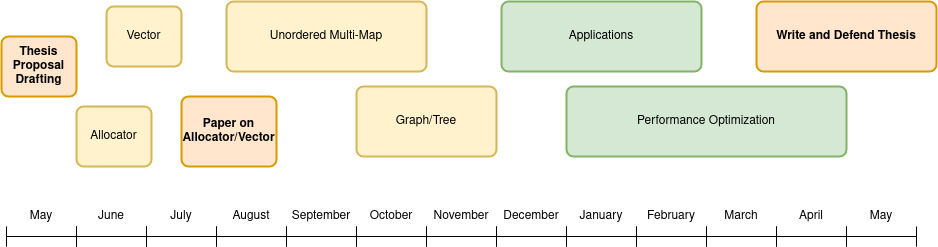
\includegraphics[width=0.65\textwidth]{Figures/thesis_timeline.jpg}
\caption{Thesis timeline}
\label{fig:thesis_timeline}
\end{figure}



\section{Dissemination of Results}
We plan to split the results into two separate sections: an initial paper, which will cover the details of \texttt{pc2l::vector} and \texttt{pc2l::allocator}, and the full thesis, which will cover the complete implementation, optimization, and application of all data structures in PC2L. We will submit abstracts/drafts of the final thesis paper to the ACM Symposium on the Principles of Distributed Computing, IEEE International Parallel and Distributed Processing Symposium, and the ACM International Symposium on High Performance Distributed Computing. We will submit the paper on \texttt{pc2l::allocator} and \texttt{pc2l::vector} to IEEE Transactions on Parallel and Distributed Systems (TDPS), Springer's Distributed Computing, and Elsevir's Journal of Parallel and Distributed Computing. All of these submissions will be standard journal articles. Additionally, the complete thesis will be published to OhioLink, as is standard for graduate theses from this department.

\section{Validation}

While PC2L may sound great so far, we are in desperate need of some objective measurables that can demonstrate its efficiency, scalability, and usability. The goal will be to maximize each of these three key attributes, hopefully enough that they exceed comparable measurements for competing libraries. 


\subsection{Performance Comparison with Sequential Equivalents}
First, we will compare PC2L data structures with their sequential equivalents in the C++ STL. We will do this through several unit tests which fill, remove, and find elements within several of PC2L's data structures. Of course, some data structures, like the \texttt{pc2l::graph} will not have an exact sequential counterpart, in which case they will be compared to any data structure with common features, or reference libraries that implement the same structures. We expect sequential data structures to beat PC2L when a smaller number of elements is inserted into a data structure, but we expected PC2L to prevail as the number of elements in a data structure grows. 

\subsection{Adaptivity Assessment}
Users will be able to customize  caching in PC2L such that the elements that are cached best suit the access pattern of their project. In an attempt to evaluate whether this feature is actually adaptive to different access patterns, we will test different access patterns against different feature settings. For example, we could test a sequential access pattern against sequential caching, then test a regional access pattern against sequential caching, and so on and so forth. Ideally, we expect these tests to demonstrate that PC2L offers better performance when a user specifies the access pattern for their data structure. 

\subsection{Scalability Measurement}
In order to ensure that PC2L works at scale, we will put it through several different tests. First of all, we will generate several benchmark programs that are data-intensive. Finally, we will measure how the performance of each of these programs changes as nodes, processor cores, and memory are added to a run of PC2L. If designed properly, we expect PC2L to deliver better performance with each additional resource it is given. Additionally, this sort of testing can support the development process as we can graph program performance and identify if PC2L ever runs into a performance plateau after adding any number of additional resources.

\subsection{Usability Measurement}
Above all, PC2L is a library designed for user consumption. Any library we make will be essentially useless outside of our lab unless we can convince real users to adopt it. This is where our measurement of usability comes in. After PC2L is fully develop, we will find both experienced and novice distributed computing developers, hand them the documentation, and have them evaluate how usable PC2L is across several different criteria. There are several different major usability metrics that come up in \cite{use} including efficiency, effectiveness, productivity, satisfaction, learnability, safety, trustfulness, accessibility, and usefulness. While these criteria are typically used for non-technical, consumer-facing products, we can adapt some of them for our purposes


\subsection{Stopping Criteria}
Although all of these evaluation criteria are important, the main metric we will use to determine a stopping point will be performance and scalability. We have made this choice because although changing syntax and/or adaptability features will be trivial once the full implementation is complete, changing core features will not be so easy. With this in mind, we will leave achieving ideal usability and adaptivity to future researchers, and instead focus on achieving similar, if not better, scalability and performance when compared with other frameworks. More specifically, PC2L will be complete when it can compete with and/or beat competing distributed computing frameworks in stress test utilizing memory-intensive, big memory applications. 


